\section{程式架構}
\label{app:architecture}

\subsection{系統架構}

圖~\ref{fig:c4-component} 以 C4 model 的 Component 層級描述 Graphtoria。使用者的輸入經 FreeGLUT 轉為 callback，由 GUI Framework（附錄~\ref{app:gui}）分派給 Canvas；Canvas 將輸入交給目前的 Tool，再依 Tool 回傳的結果修改 Document。Renderers 負責第~\ref{sec:stroke-geometry}--\ref{sec:gfnt-render} 節的繪製，IO 則負責 GPTD 文件的讀寫與 PPM 匯出。

\begin{figure}[htbp]
    \centering
    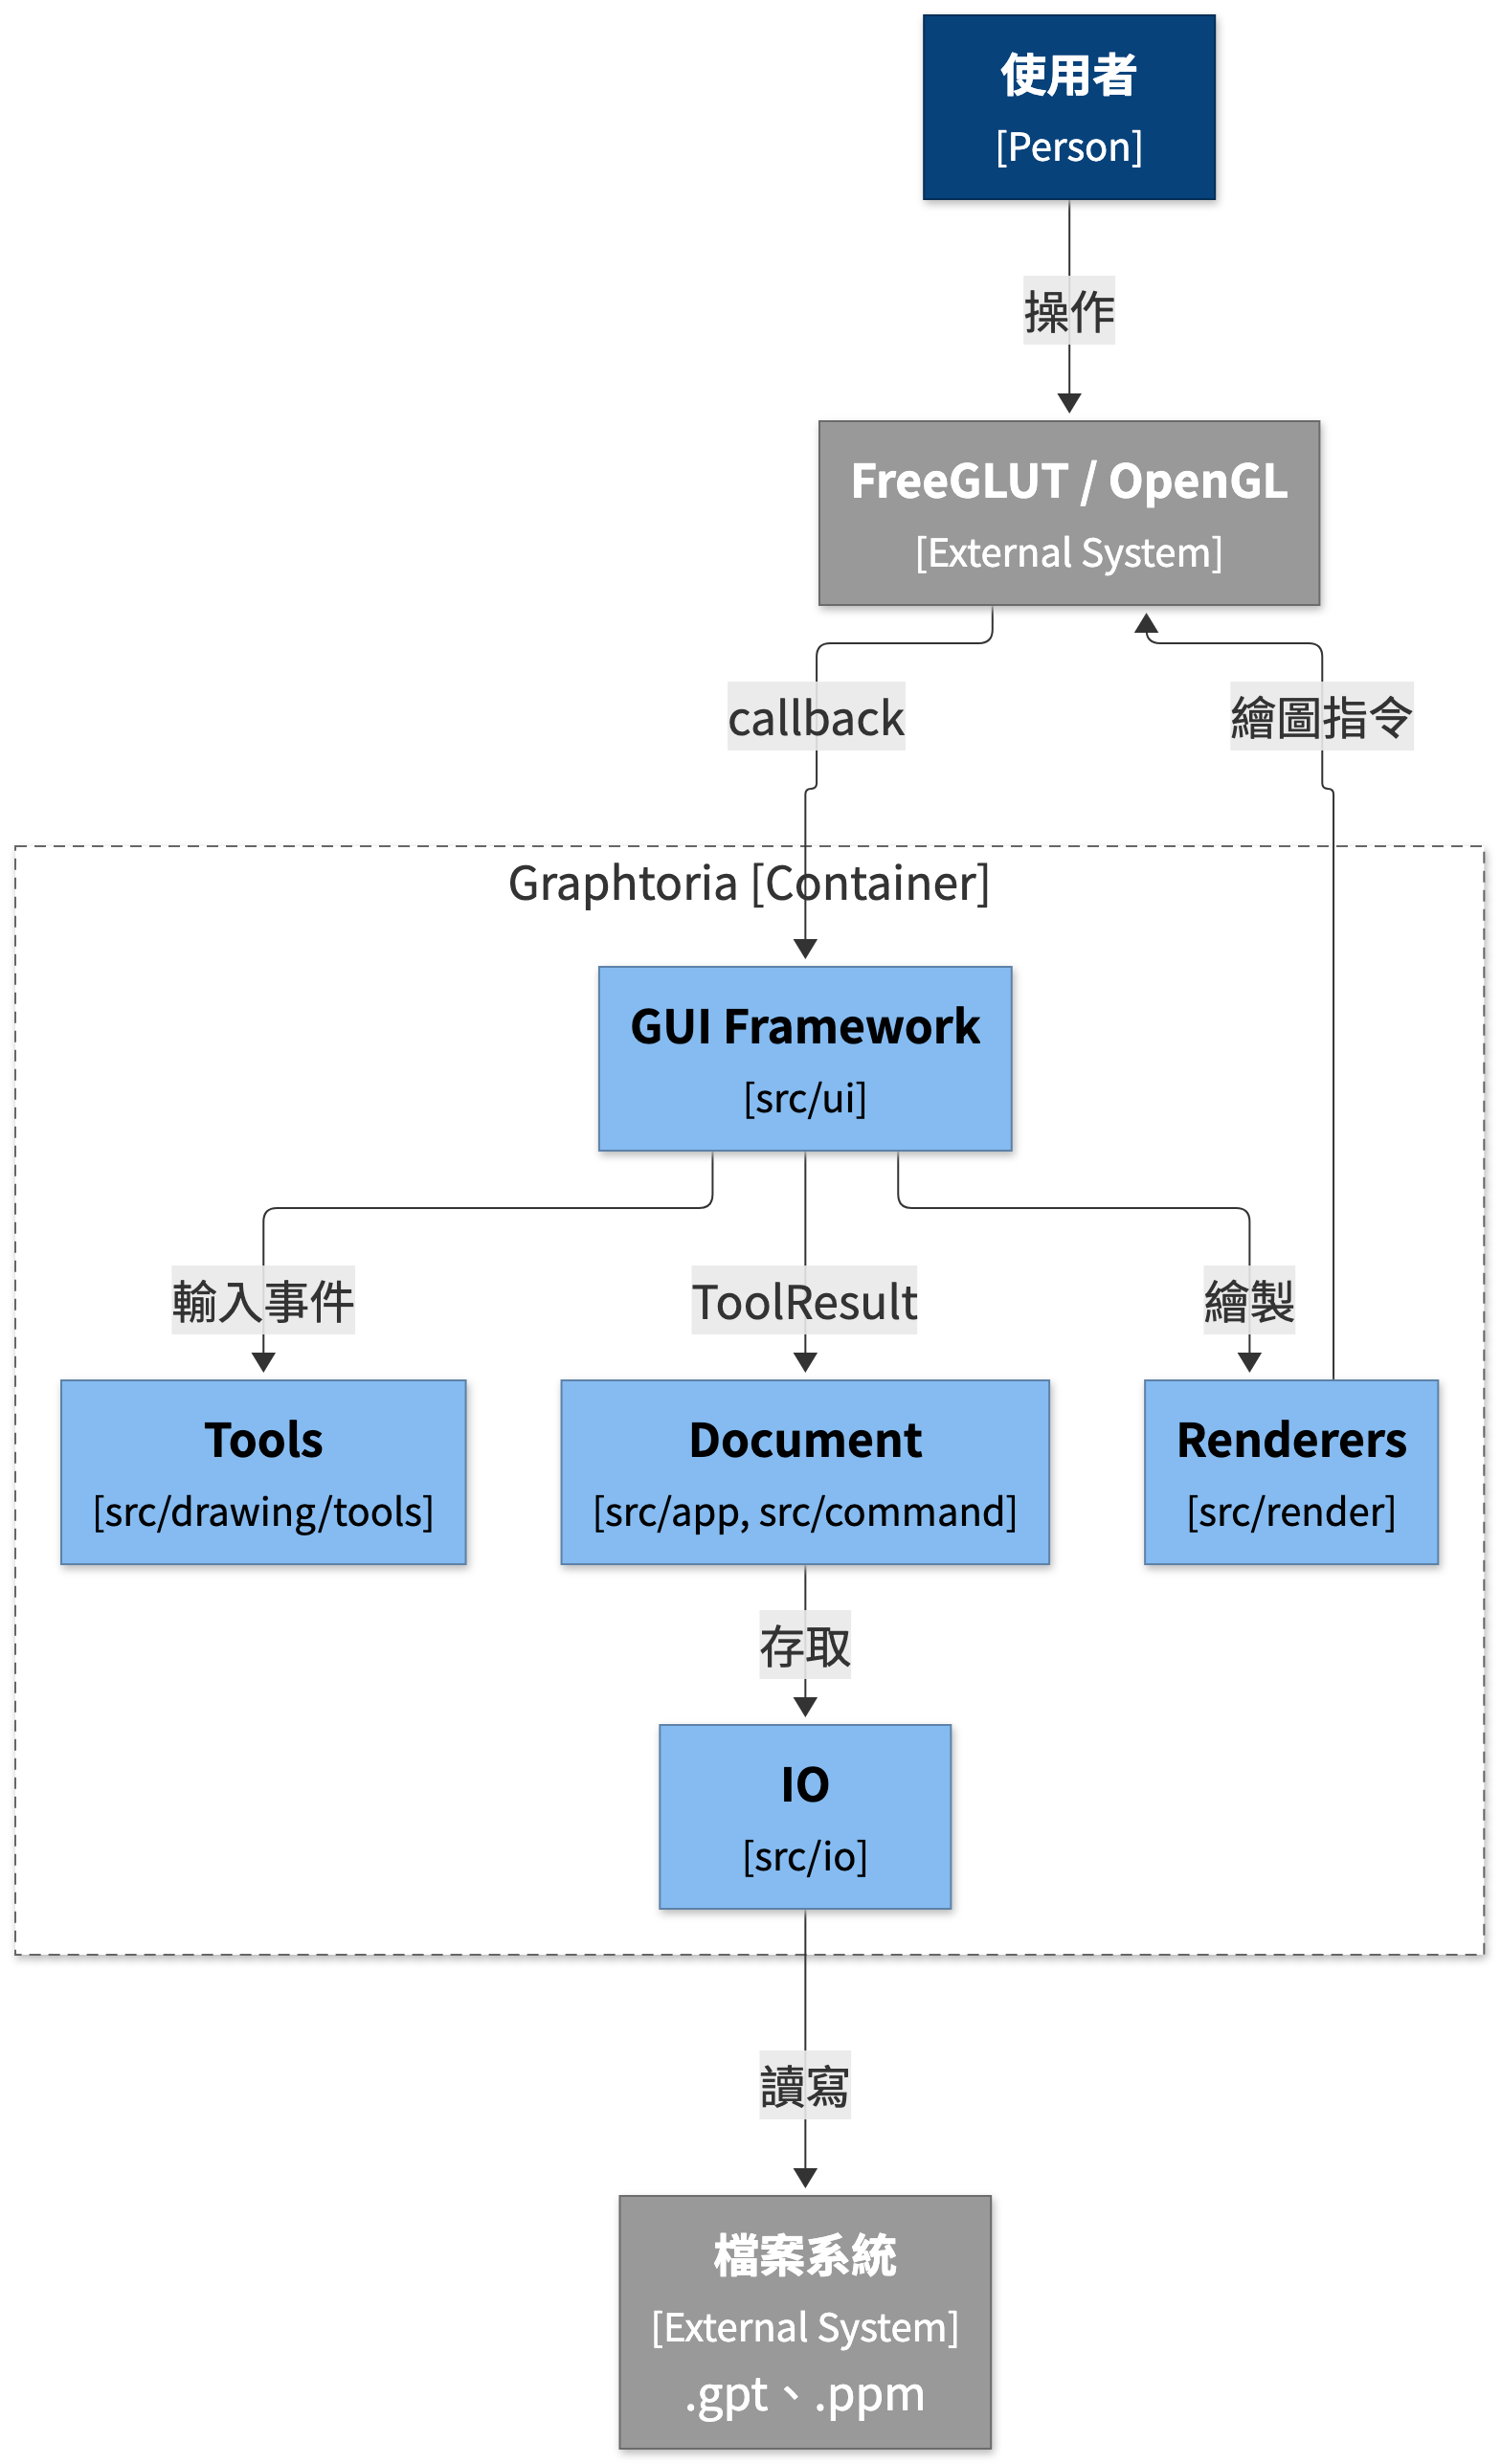
\includegraphics[width=.5\textwidth]{docs/figures/app_c_c4-component.png}
    \caption{Graphtoria 的 C4 Component 圖}
    \label{fig:c4-component}
\end{figure}

\subsection{資料模型}

Document 擁有 Scene 與 CommandHistory，如圖~\ref{fig:class-command}。Scene 依繪製順序保存 SceneObject，其繼承關係如圖~\ref{fig:class-scene}：Shape 依幾何分為單點、兩點決定的圖形與頂點序列，對應第~\ref{sec:geometry-representation} 節的幾何表示。對 Scene 的每一種修改都包裝成可 \lstinline|execute()| 與 \lstinline|undo()| 的 Command，目前有新增、插入、刪除與清空四種，由 CommandHistory 以 undo 與 redo 兩個堆疊管理。每執行一個 Command 都會產生新的狀態編號，與存檔時的編號比較，即可判斷文件是否有未儲存的變更；因此修改後再 Undo 回存檔時的狀態，也會正確視為未修改。

\begin{figure}[htbp]
    \centering
    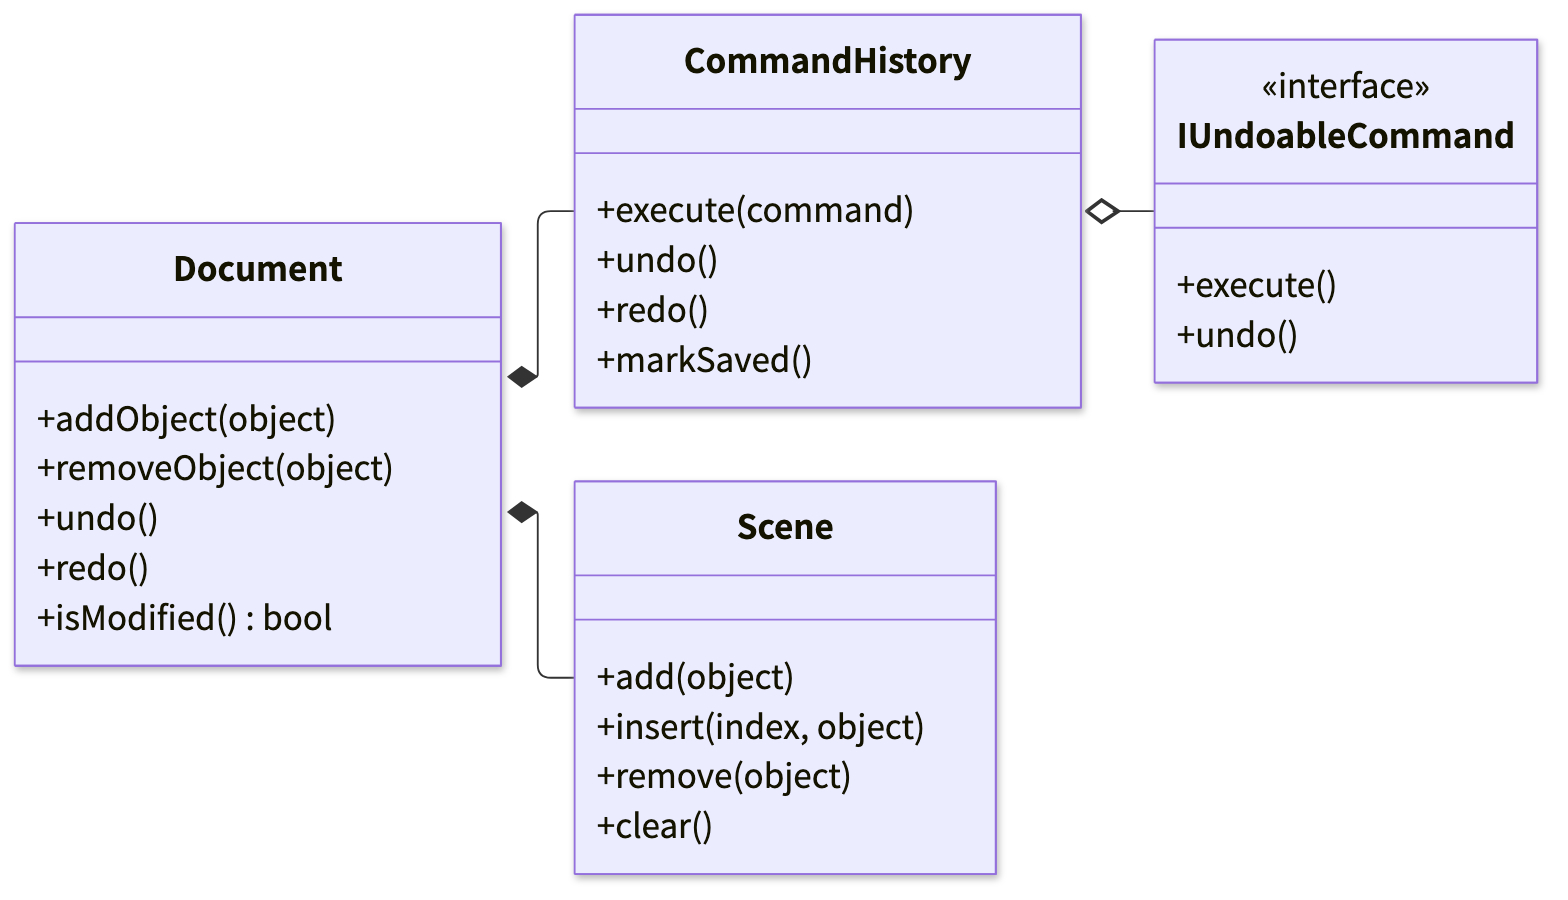
\includegraphics[width=.6\textwidth]{docs/figures/app_c_class-command.png}
    \caption{Document 與 Command 的類別圖}
    \label{fig:class-command}
\end{figure}

\begin{figure}[htbp]
    \centering
    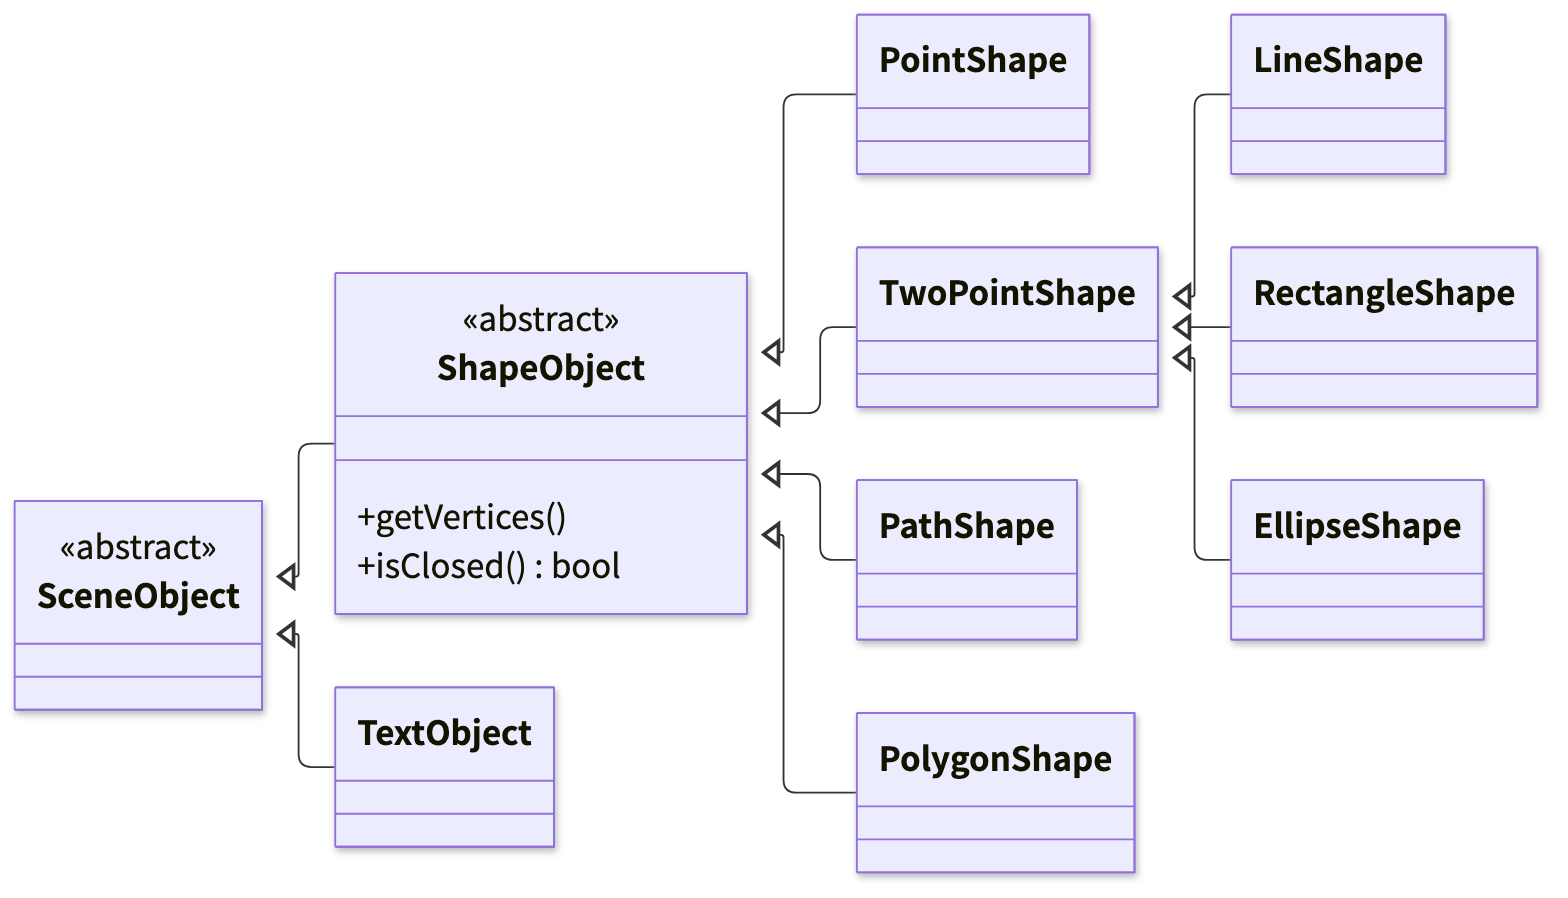
\includegraphics[width=.6\textwidth]{docs/figures/app_c_class-scene.png}
    \caption{Scene 物件的類別圖}
    \label{fig:class-scene}
\end{figure}

\subsection{繪圖工具}

所有工具實作 \lstinline|ICanvasTool|，如圖~\ref{fig:class-tools}。工具不直接修改 Document，而是回傳 \lstinline|ToolResult|，描述是否需要重畫，以及要新增、刪除物件或開啟文字輸入框，由 CanvasElement 統一執行。會建立圖形的工具共用 \lstinline|CreationTool| 的 Draft 管理（第~\ref{sec:draft} 節）；拖曳類工具再共用 \lstinline|DragTool| 的起點、終點與 Shift 限制邏輯。

\begin{figure}[htbp]
    \centering
    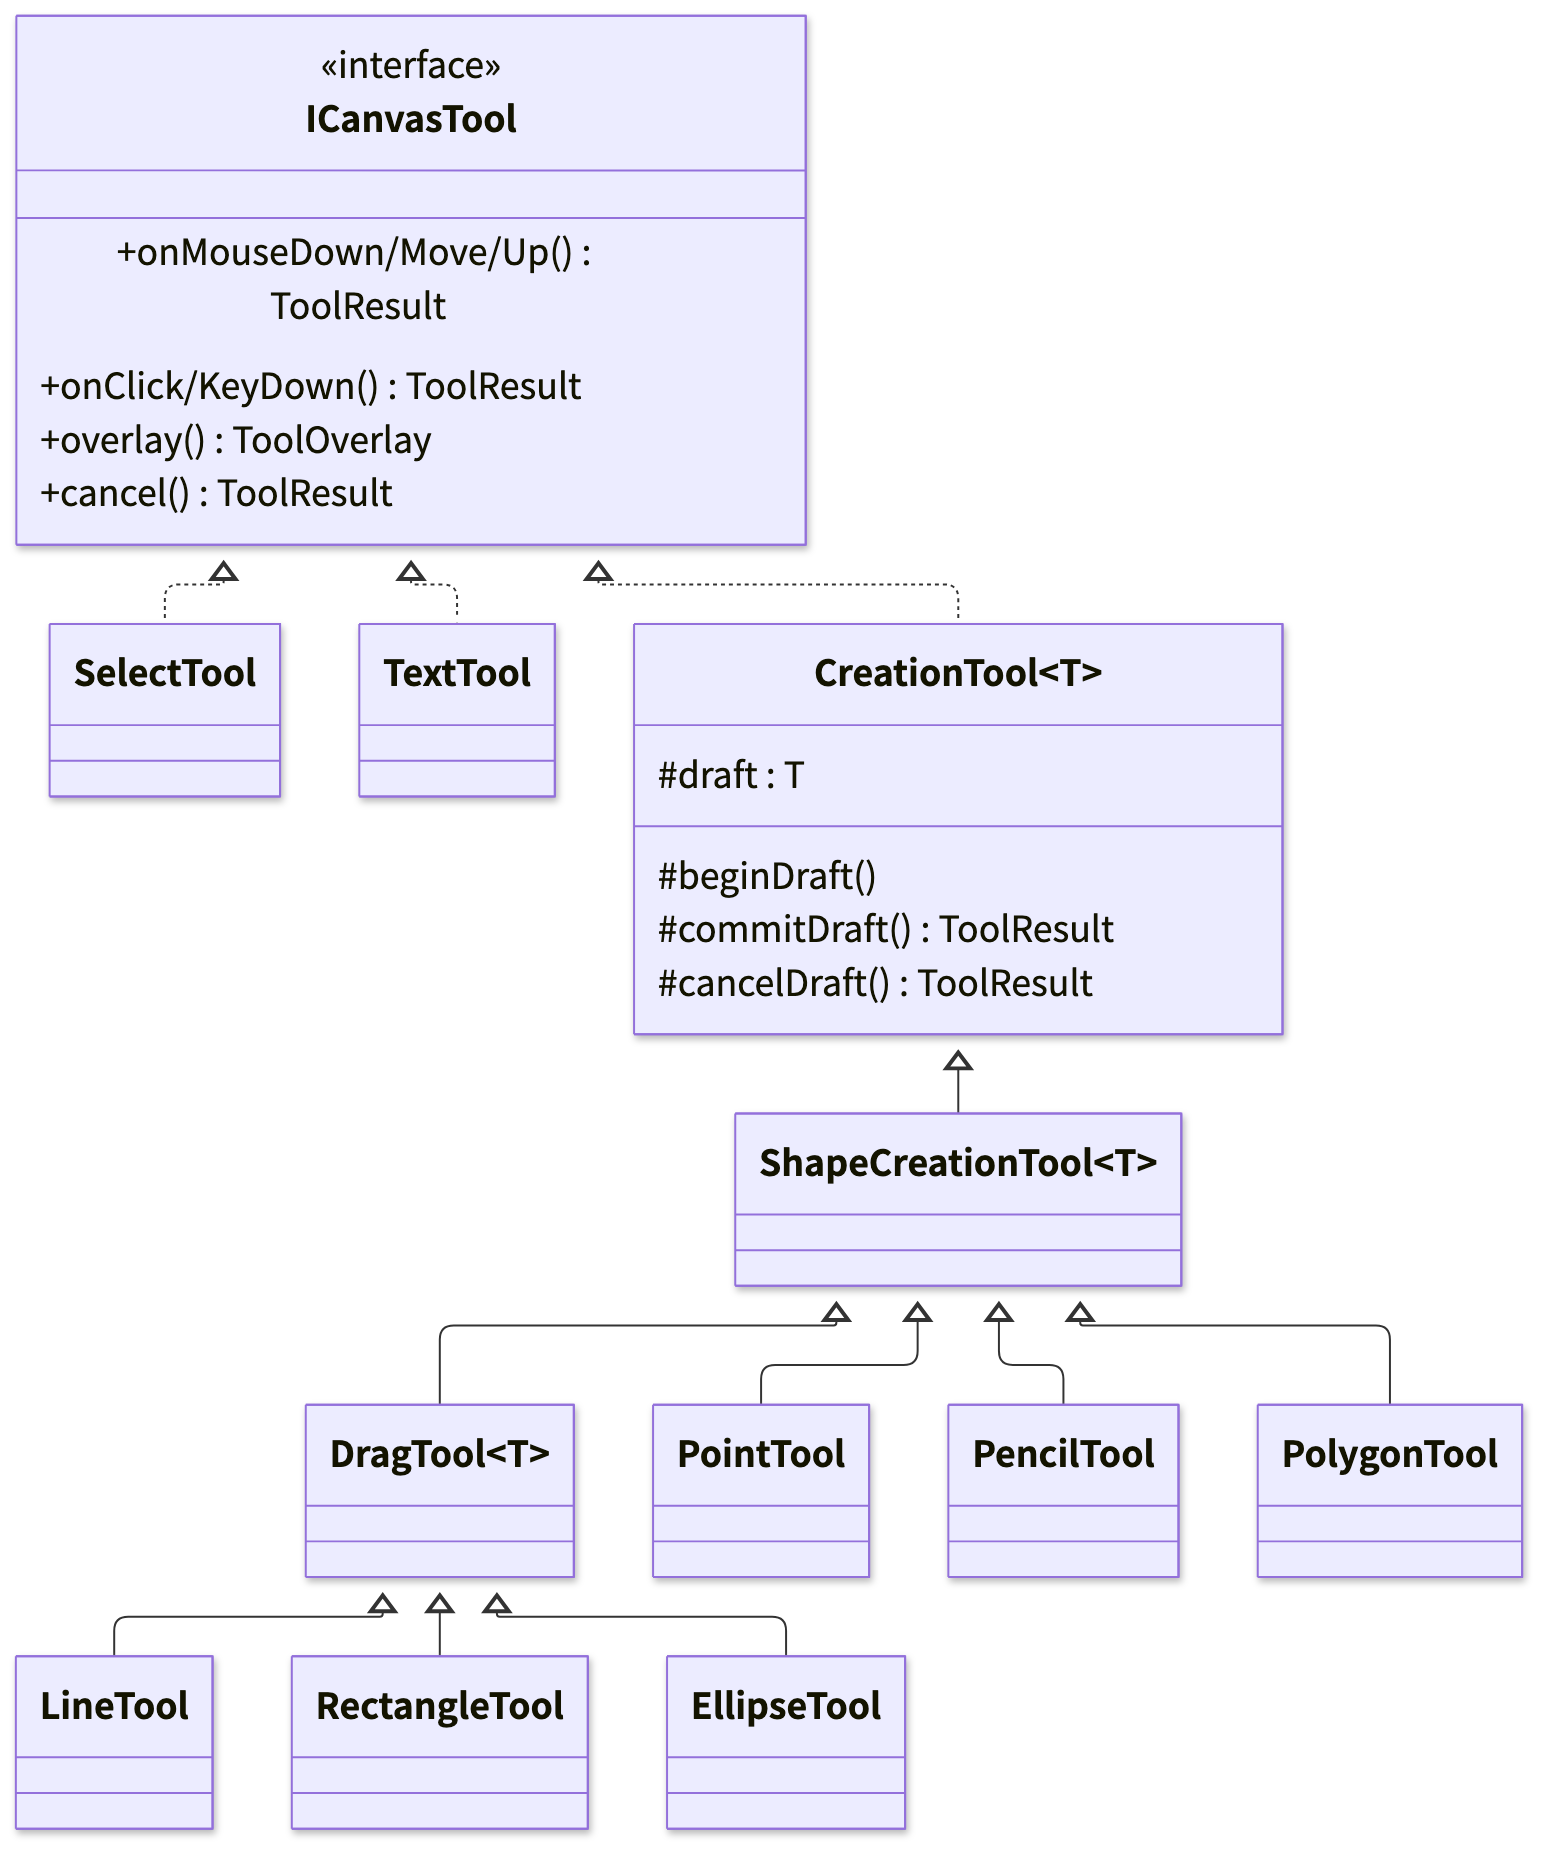
\includegraphics[width=.5\textwidth]{docs/figures/app_c_class-tools.png}
    \caption{繪圖工具的類別圖}
    \label{fig:class-tools}
\end{figure}

\subsection{繪製一條直線的流程}

圖~\ref{fig:sequence-line} 以 Line 工具為例串起上述元件：按下滑鼠時 Canvas 取得 mouse capture，拖曳中工具只更新 Draft，放開後 Canvas 才將新增物件的動作交給 Document 包裝成 Command 執行。

\begin{figure}[htbp]
    \centering
    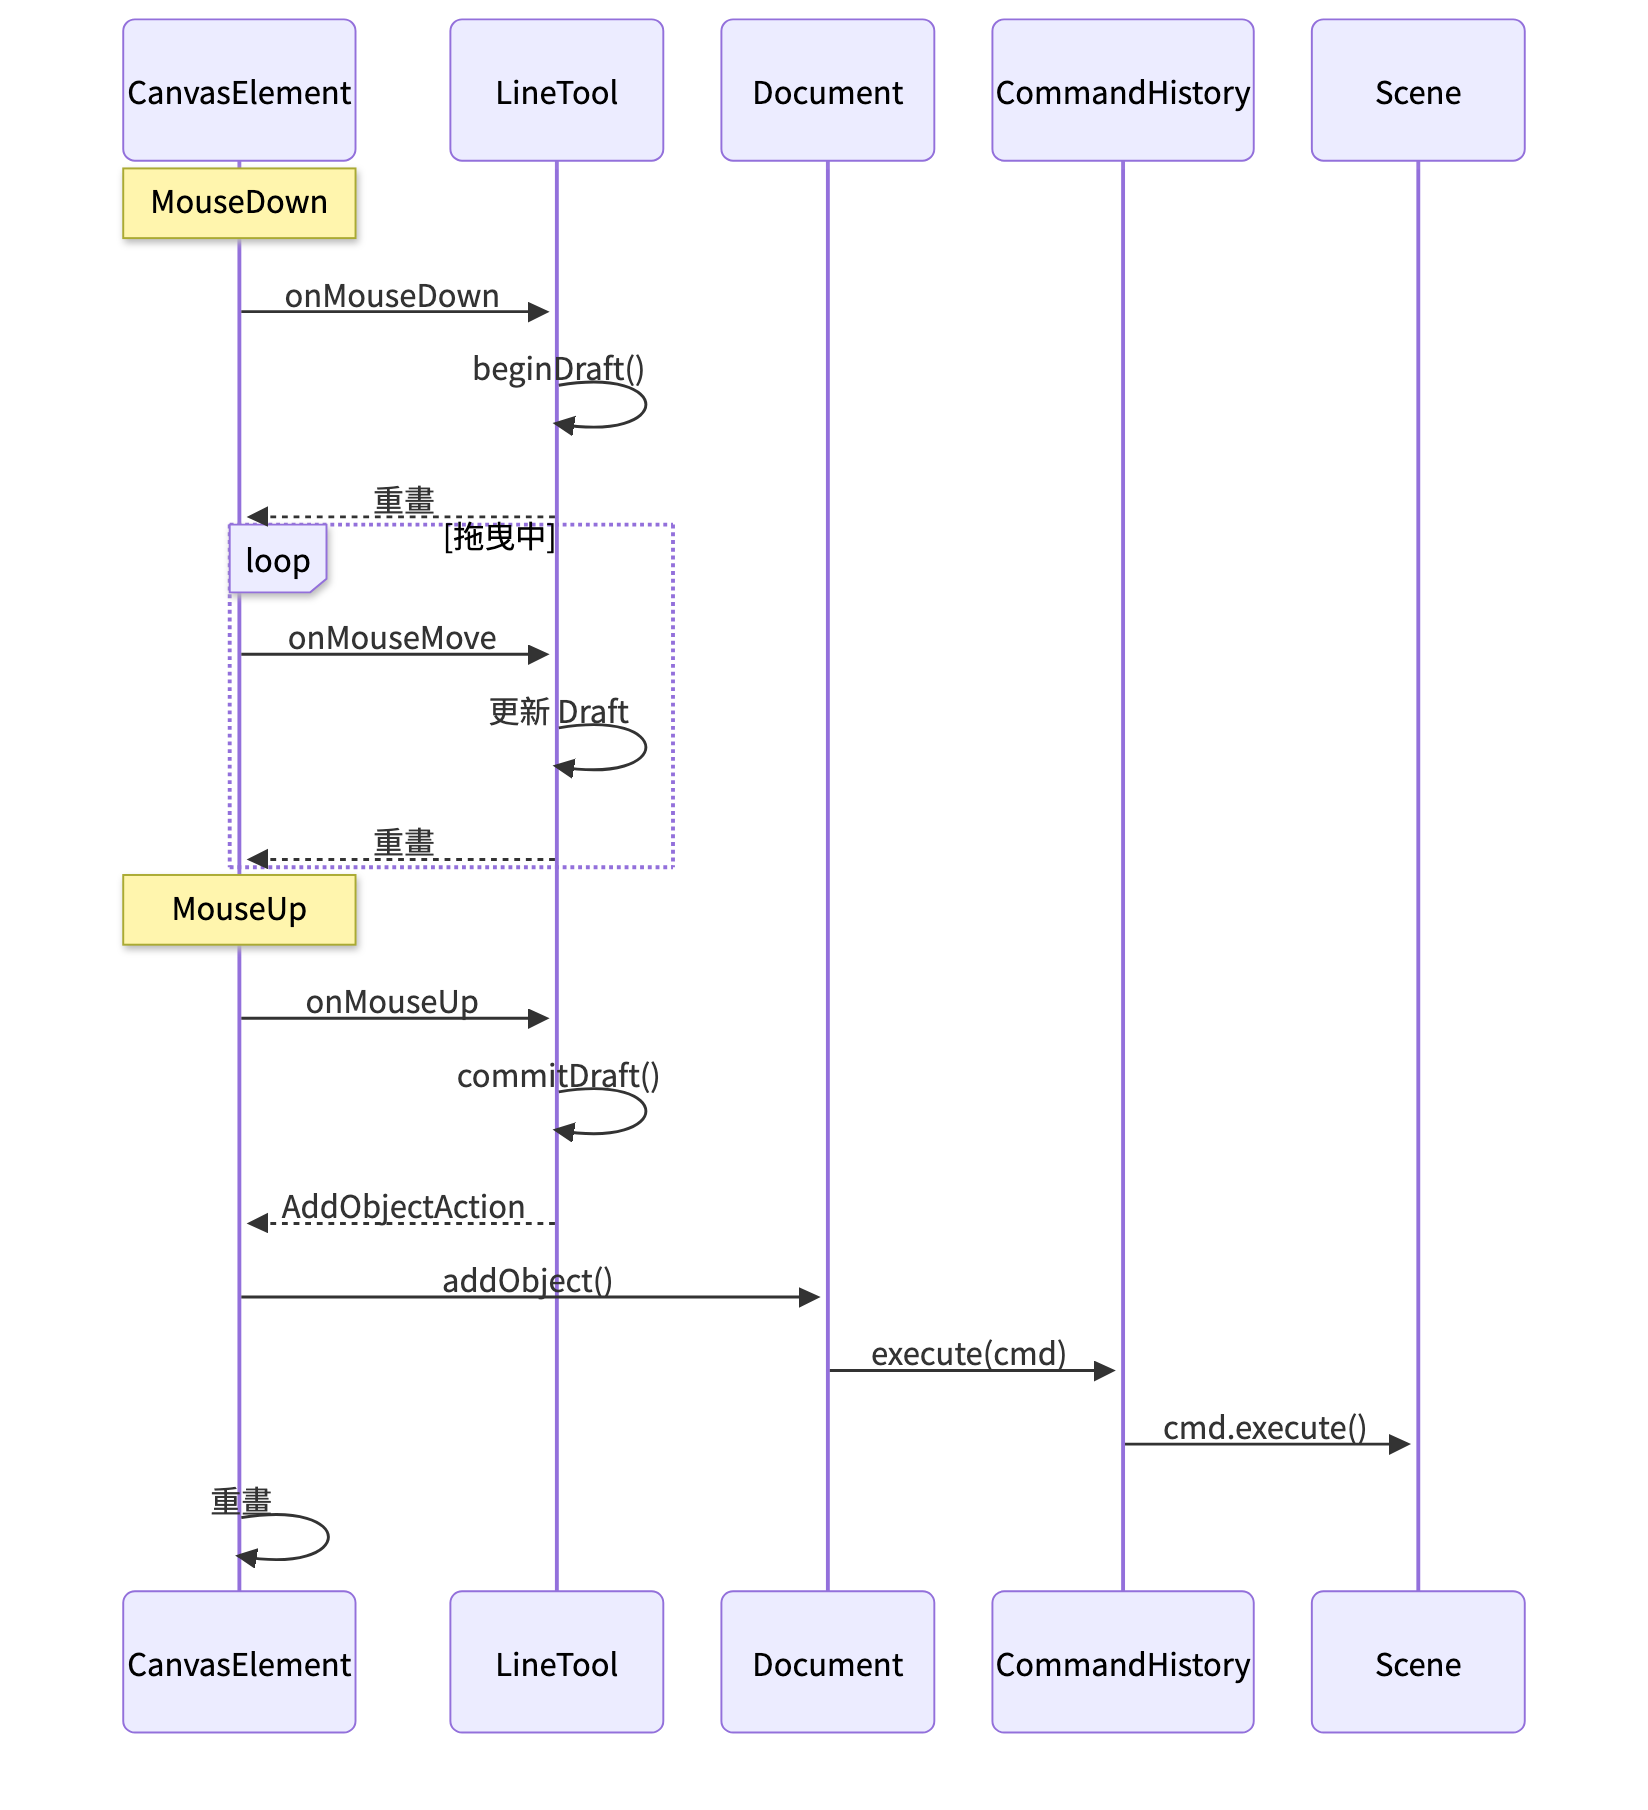
\includegraphics[width=.85\textwidth]{docs/figures/app_c_sequence-line.png}
    \caption{以 Line 工具繪製一條直線的循序圖}
    \label{fig:sequence-line}
\end{figure}
